% Options for packages loaded elsewhere
\PassOptionsToPackage{unicode}{hyperref}
\PassOptionsToPackage{hyphens}{url}
\PassOptionsToPackage{dvipsnames,svgnames,x11names}{xcolor}
%
\documentclass[
  letterpaper,
  DIV=11,
  numbers=noendperiod]{scrreprt}

\usepackage{amsmath,amssymb}
\usepackage{iftex}
\ifPDFTeX
  \usepackage[T1]{fontenc}
  \usepackage[utf8]{inputenc}
  \usepackage{textcomp} % provide euro and other symbols
\else % if luatex or xetex
  \usepackage{unicode-math}
  \defaultfontfeatures{Scale=MatchLowercase}
  \defaultfontfeatures[\rmfamily]{Ligatures=TeX,Scale=1}
\fi
\usepackage{lmodern}
\ifPDFTeX\else  
    % xetex/luatex font selection
\fi
% Use upquote if available, for straight quotes in verbatim environments
\IfFileExists{upquote.sty}{\usepackage{upquote}}{}
\IfFileExists{microtype.sty}{% use microtype if available
  \usepackage[]{microtype}
  \UseMicrotypeSet[protrusion]{basicmath} % disable protrusion for tt fonts
}{}
\makeatletter
\@ifundefined{KOMAClassName}{% if non-KOMA class
  \IfFileExists{parskip.sty}{%
    \usepackage{parskip}
  }{% else
    \setlength{\parindent}{0pt}
    \setlength{\parskip}{6pt plus 2pt minus 1pt}}
}{% if KOMA class
  \KOMAoptions{parskip=half}}
\makeatother
\usepackage{xcolor}
\setlength{\emergencystretch}{3em} % prevent overfull lines
\setcounter{secnumdepth}{5}
% Make \paragraph and \subparagraph free-standing
\ifx\paragraph\undefined\else
  \let\oldparagraph\paragraph
  \renewcommand{\paragraph}[1]{\oldparagraph{#1}\mbox{}}
\fi
\ifx\subparagraph\undefined\else
  \let\oldsubparagraph\subparagraph
  \renewcommand{\subparagraph}[1]{\oldsubparagraph{#1}\mbox{}}
\fi

\usepackage{color}
\usepackage{fancyvrb}
\newcommand{\VerbBar}{|}
\newcommand{\VERB}{\Verb[commandchars=\\\{\}]}
\DefineVerbatimEnvironment{Highlighting}{Verbatim}{commandchars=\\\{\}}
% Add ',fontsize=\small' for more characters per line
\usepackage{framed}
\definecolor{shadecolor}{RGB}{241,243,245}
\newenvironment{Shaded}{\begin{snugshade}}{\end{snugshade}}
\newcommand{\AlertTok}[1]{\textcolor[rgb]{0.68,0.00,0.00}{#1}}
\newcommand{\AnnotationTok}[1]{\textcolor[rgb]{0.37,0.37,0.37}{#1}}
\newcommand{\AttributeTok}[1]{\textcolor[rgb]{0.40,0.45,0.13}{#1}}
\newcommand{\BaseNTok}[1]{\textcolor[rgb]{0.68,0.00,0.00}{#1}}
\newcommand{\BuiltInTok}[1]{\textcolor[rgb]{0.00,0.23,0.31}{#1}}
\newcommand{\CharTok}[1]{\textcolor[rgb]{0.13,0.47,0.30}{#1}}
\newcommand{\CommentTok}[1]{\textcolor[rgb]{0.37,0.37,0.37}{#1}}
\newcommand{\CommentVarTok}[1]{\textcolor[rgb]{0.37,0.37,0.37}{\textit{#1}}}
\newcommand{\ConstantTok}[1]{\textcolor[rgb]{0.56,0.35,0.01}{#1}}
\newcommand{\ControlFlowTok}[1]{\textcolor[rgb]{0.00,0.23,0.31}{#1}}
\newcommand{\DataTypeTok}[1]{\textcolor[rgb]{0.68,0.00,0.00}{#1}}
\newcommand{\DecValTok}[1]{\textcolor[rgb]{0.68,0.00,0.00}{#1}}
\newcommand{\DocumentationTok}[1]{\textcolor[rgb]{0.37,0.37,0.37}{\textit{#1}}}
\newcommand{\ErrorTok}[1]{\textcolor[rgb]{0.68,0.00,0.00}{#1}}
\newcommand{\ExtensionTok}[1]{\textcolor[rgb]{0.00,0.23,0.31}{#1}}
\newcommand{\FloatTok}[1]{\textcolor[rgb]{0.68,0.00,0.00}{#1}}
\newcommand{\FunctionTok}[1]{\textcolor[rgb]{0.28,0.35,0.67}{#1}}
\newcommand{\ImportTok}[1]{\textcolor[rgb]{0.00,0.46,0.62}{#1}}
\newcommand{\InformationTok}[1]{\textcolor[rgb]{0.37,0.37,0.37}{#1}}
\newcommand{\KeywordTok}[1]{\textcolor[rgb]{0.00,0.23,0.31}{#1}}
\newcommand{\NormalTok}[1]{\textcolor[rgb]{0.00,0.23,0.31}{#1}}
\newcommand{\OperatorTok}[1]{\textcolor[rgb]{0.37,0.37,0.37}{#1}}
\newcommand{\OtherTok}[1]{\textcolor[rgb]{0.00,0.23,0.31}{#1}}
\newcommand{\PreprocessorTok}[1]{\textcolor[rgb]{0.68,0.00,0.00}{#1}}
\newcommand{\RegionMarkerTok}[1]{\textcolor[rgb]{0.00,0.23,0.31}{#1}}
\newcommand{\SpecialCharTok}[1]{\textcolor[rgb]{0.37,0.37,0.37}{#1}}
\newcommand{\SpecialStringTok}[1]{\textcolor[rgb]{0.13,0.47,0.30}{#1}}
\newcommand{\StringTok}[1]{\textcolor[rgb]{0.13,0.47,0.30}{#1}}
\newcommand{\VariableTok}[1]{\textcolor[rgb]{0.07,0.07,0.07}{#1}}
\newcommand{\VerbatimStringTok}[1]{\textcolor[rgb]{0.13,0.47,0.30}{#1}}
\newcommand{\WarningTok}[1]{\textcolor[rgb]{0.37,0.37,0.37}{\textit{#1}}}

\providecommand{\tightlist}{%
  \setlength{\itemsep}{0pt}\setlength{\parskip}{0pt}}\usepackage{longtable,booktabs,array}
\usepackage{calc} % for calculating minipage widths
% Correct order of tables after \paragraph or \subparagraph
\usepackage{etoolbox}
\makeatletter
\patchcmd\longtable{\par}{\if@noskipsec\mbox{}\fi\par}{}{}
\makeatother
% Allow footnotes in longtable head/foot
\IfFileExists{footnotehyper.sty}{\usepackage{footnotehyper}}{\usepackage{footnote}}
\makesavenoteenv{longtable}
\usepackage{graphicx}
\makeatletter
\def\maxwidth{\ifdim\Gin@nat@width>\linewidth\linewidth\else\Gin@nat@width\fi}
\def\maxheight{\ifdim\Gin@nat@height>\textheight\textheight\else\Gin@nat@height\fi}
\makeatother
% Scale images if necessary, so that they will not overflow the page
% margins by default, and it is still possible to overwrite the defaults
% using explicit options in \includegraphics[width, height, ...]{}
\setkeys{Gin}{width=\maxwidth,height=\maxheight,keepaspectratio}
% Set default figure placement to htbp
\makeatletter
\def\fps@figure{htbp}
\makeatother

\KOMAoption{captions}{tableheading}
\makeatletter
\@ifpackageloaded{tcolorbox}{}{\usepackage[skins,breakable]{tcolorbox}}
\@ifpackageloaded{fontawesome5}{}{\usepackage{fontawesome5}}
\definecolor{quarto-callout-color}{HTML}{909090}
\definecolor{quarto-callout-note-color}{HTML}{0758E5}
\definecolor{quarto-callout-important-color}{HTML}{CC1914}
\definecolor{quarto-callout-warning-color}{HTML}{EB9113}
\definecolor{quarto-callout-tip-color}{HTML}{00A047}
\definecolor{quarto-callout-caution-color}{HTML}{FC5300}
\definecolor{quarto-callout-color-frame}{HTML}{acacac}
\definecolor{quarto-callout-note-color-frame}{HTML}{4582ec}
\definecolor{quarto-callout-important-color-frame}{HTML}{d9534f}
\definecolor{quarto-callout-warning-color-frame}{HTML}{f0ad4e}
\definecolor{quarto-callout-tip-color-frame}{HTML}{02b875}
\definecolor{quarto-callout-caution-color-frame}{HTML}{fd7e14}
\makeatother
\makeatletter
\makeatother
\makeatletter
\makeatother
\makeatletter
\@ifpackageloaded{caption}{}{\usepackage{caption}}
\AtBeginDocument{%
\ifdefined\contentsname
  \renewcommand*\contentsname{Table of contents}
\else
  \newcommand\contentsname{Table of contents}
\fi
\ifdefined\listfigurename
  \renewcommand*\listfigurename{List of Figures}
\else
  \newcommand\listfigurename{List of Figures}
\fi
\ifdefined\listtablename
  \renewcommand*\listtablename{List of Tables}
\else
  \newcommand\listtablename{List of Tables}
\fi
\ifdefined\figurename
  \renewcommand*\figurename{Figure}
\else
  \newcommand\figurename{Figure}
\fi
\ifdefined\tablename
  \renewcommand*\tablename{Table}
\else
  \newcommand\tablename{Table}
\fi
}
\@ifpackageloaded{float}{}{\usepackage{float}}
\floatstyle{ruled}
\@ifundefined{c@chapter}{\newfloat{codelisting}{h}{lop}}{\newfloat{codelisting}{h}{lop}[chapter]}
\floatname{codelisting}{Listing}
\newcommand*\listoflistings{\listof{codelisting}{List of Listings}}
\makeatother
\makeatletter
\@ifpackageloaded{caption}{}{\usepackage{caption}}
\@ifpackageloaded{subcaption}{}{\usepackage{subcaption}}
\makeatother
\makeatletter
\@ifpackageloaded{tcolorbox}{}{\usepackage[skins,breakable]{tcolorbox}}
\makeatother
\makeatletter
\@ifundefined{shadecolor}{\definecolor{shadecolor}{rgb}{.97, .97, .97}}
\makeatother
\makeatletter
\makeatother
\makeatletter
\makeatother
\ifLuaTeX
  \usepackage{selnolig}  % disable illegal ligatures
\fi
\IfFileExists{bookmark.sty}{\usepackage{bookmark}}{\usepackage{hyperref}}
\IfFileExists{xurl.sty}{\usepackage{xurl}}{} % add URL line breaks if available
\urlstyle{same} % disable monospaced font for URLs
\hypersetup{
  pdfauthor={Fiorela Castillón},
  colorlinks=true,
  linkcolor={blue},
  filecolor={Maroon},
  citecolor={Blue},
  urlcolor={Blue},
  pdfcreator={LaTeX via pandoc}}

\author{Fiorela Castillón}
\date{2023-12-11}

\begin{document}
\ifdefined\Shaded\renewenvironment{Shaded}{\begin{tcolorbox}[breakable, interior hidden, enhanced, frame hidden, borderline west={3pt}{0pt}{shadecolor}, sharp corners, boxrule=0pt]}{\end{tcolorbox}}\fi

\renewcommand*\contentsname{Table of contents}
{
\hypersetup{linkcolor=}
\setcounter{tocdepth}{2}
\tableofcontents
}
\part{Getting Started}

\hypertarget{what-is-scahpy}{%
\section*{\texorpdfstring{\textbf{What is
SCAHpy?}}{What is SCAHpy?}}\label{what-is-scahpy}}
\addcontentsline{toc}{section}{\textbf{What is SCAHpy?}}

\markright{\textbf{What is SCAHpy?}}

\textbf{\emph{SCAHpy}} is an open-source Python package that facilitate
the analysis and visualization of the ouputs from atmospheric, oceaninc
and hydrological component from the Geophysical Institute of Peru
Regional Earth System Model Croco-Oasis-WRF (IGP-RESM-COW)

\begin{figure}

{\centering 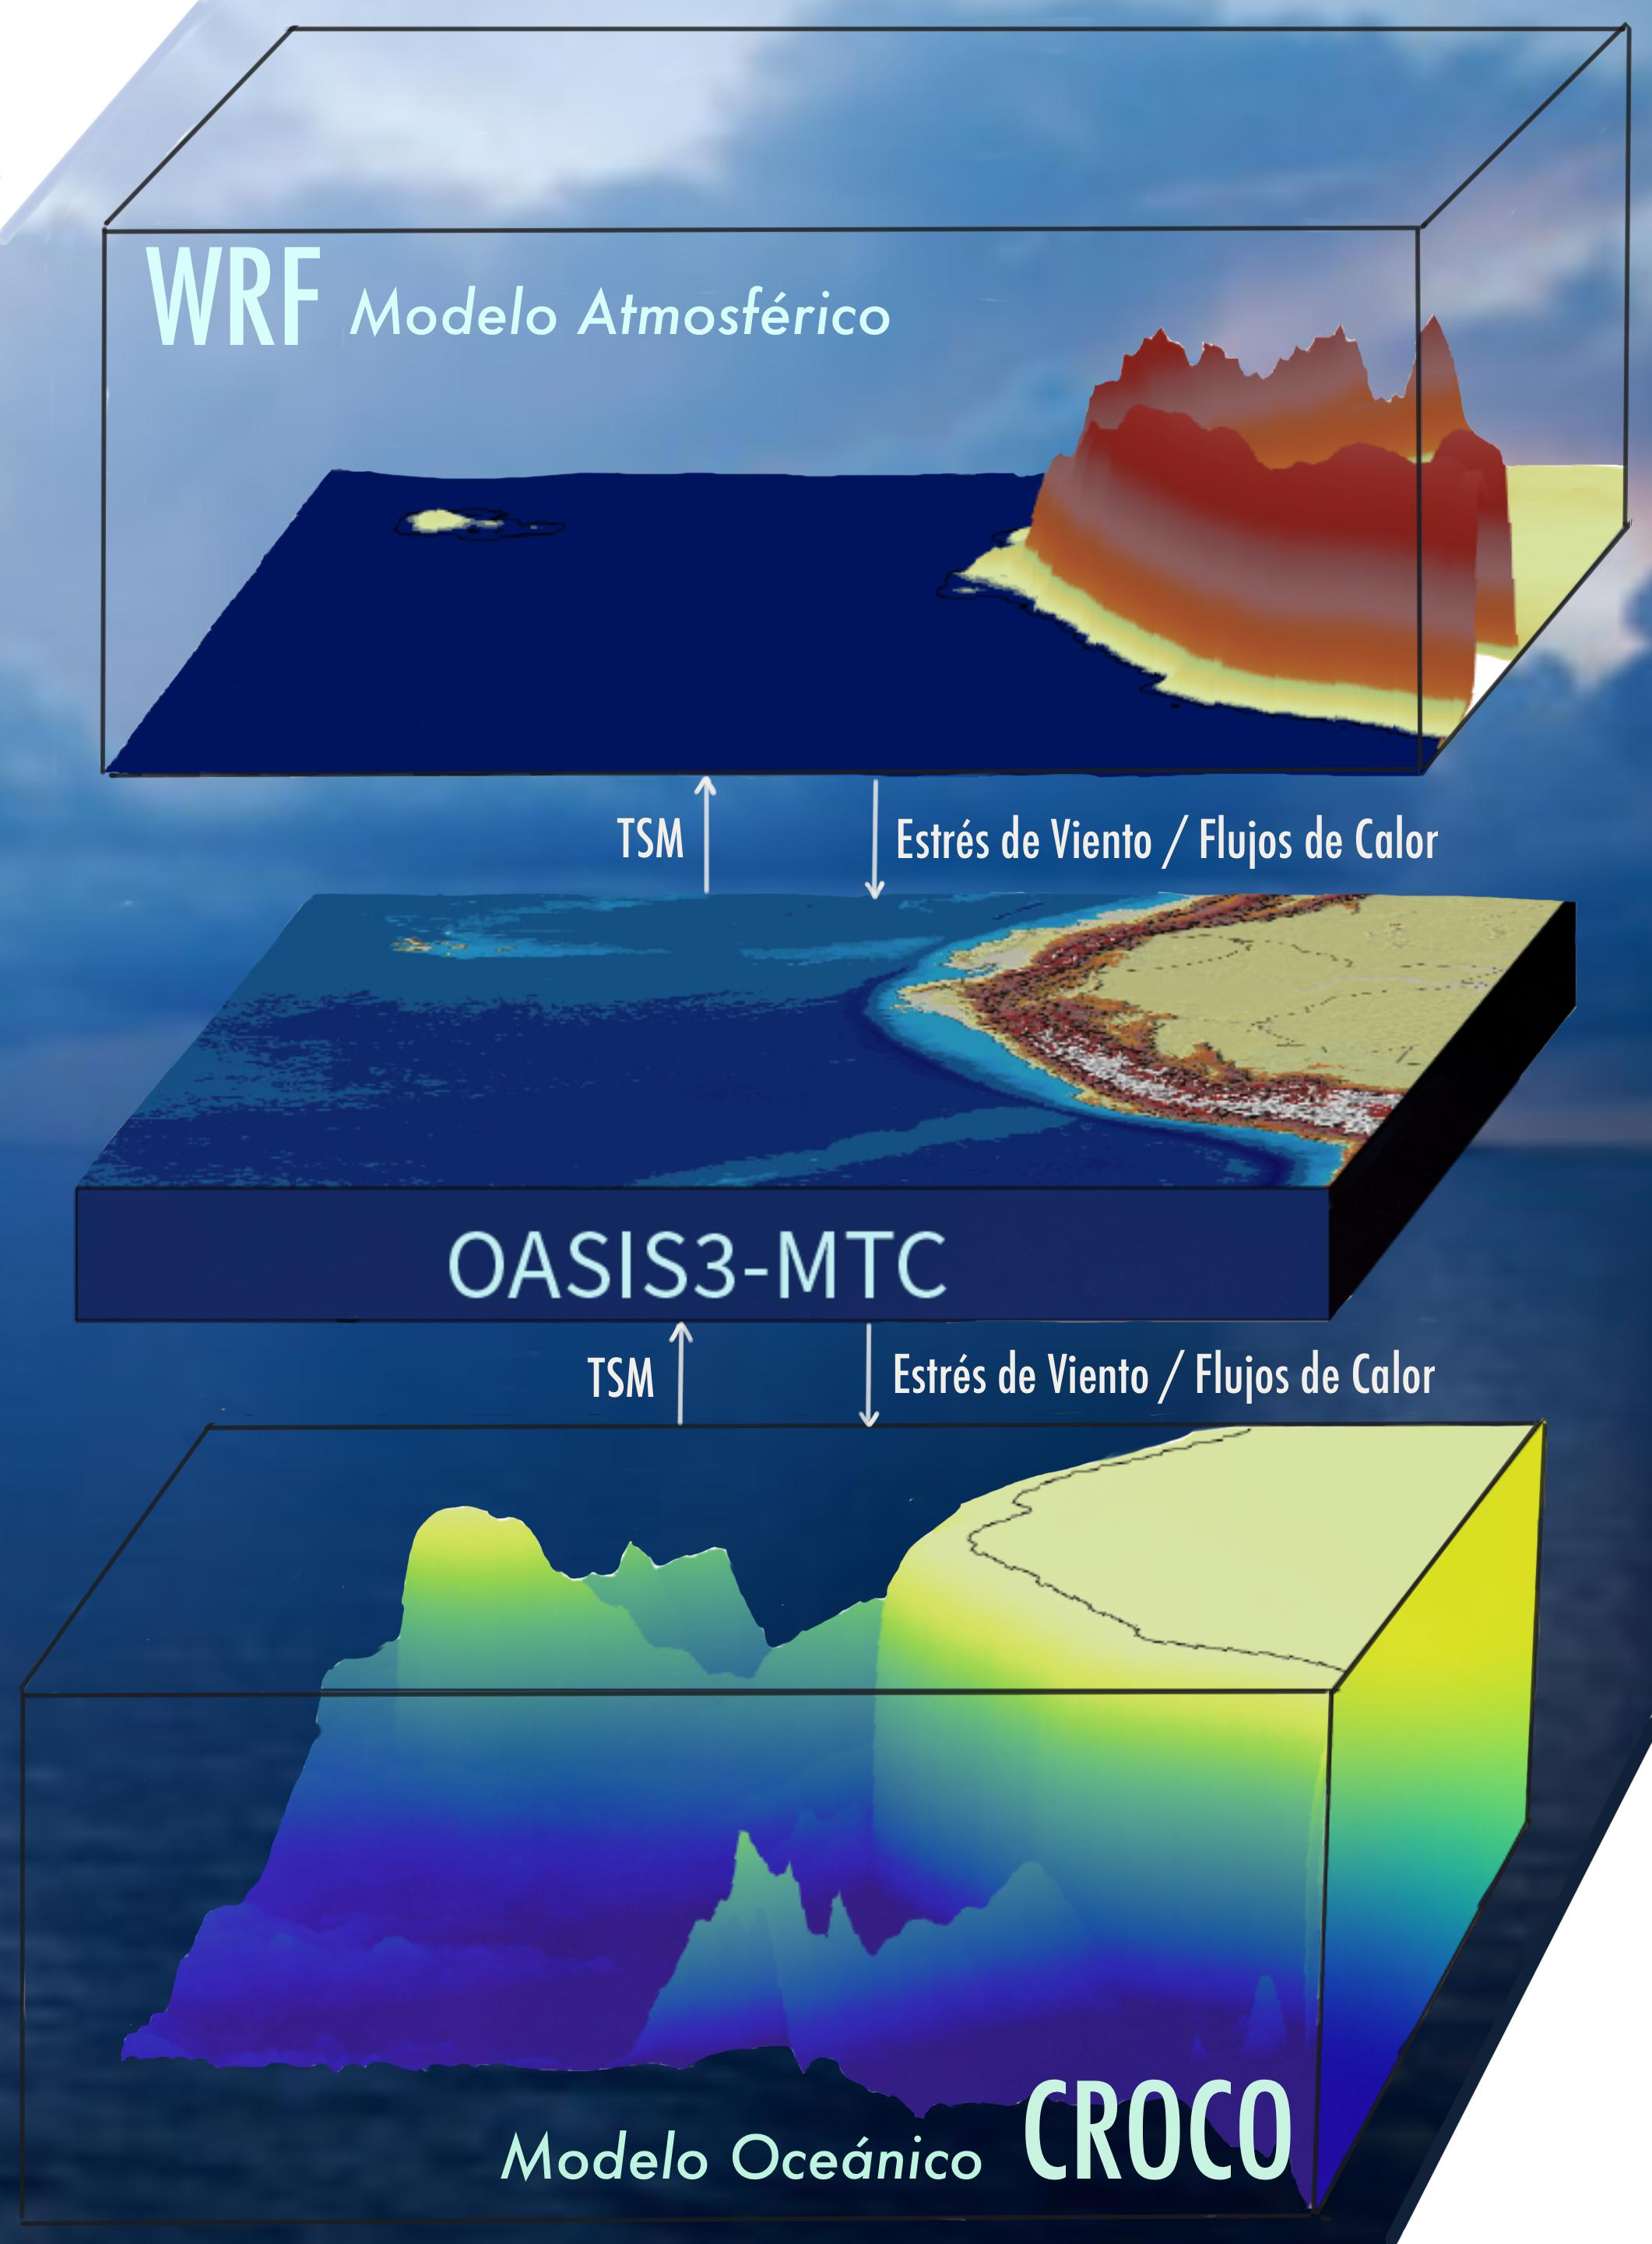
\includegraphics[width=2.85417in,height=\textheight]{cow_model.jpg}

}

\caption{COW Model - Coupled Ocean-Atmosphere Model}

\end{figure}

\hypertarget{why-is-scahpy}{%
\section*{\texorpdfstring{\textbf{Why is
SCAHpy?}}{Why is SCAHpy?}}\label{why-is-scahpy}}
\addcontentsline{toc}{section}{\textbf{Why is SCAHpy?}}

\markright{\textbf{Why is SCAHpy?}}

Atmospheric component of the coupled model generate a large volumes of
output data, making the analysis of model data harder. SCAHpy
facilitates the manage of this volumes of data, also enables a manage of
coordinates and times to local times.

\hypertarget{how-to-use-scahpy}{%
\section*{\texorpdfstring{\textbf{How to use
SCAHpy?}}{How to use SCAHpy?}}\label{how-to-use-scahpy}}
\addcontentsline{toc}{section}{\textbf{How to use SCAHpy?}}

\markright{\textbf{How to use SCAHpy?}}

SCAHpy can be used as a standalone package or it can also be run on the
HPC-IGP-Cluster, which has the diagnostic simulations of 22 years of
runnings centered on Peru Region.

\begin{tcolorbox}[enhanced jigsaw, breakable, opacitybacktitle=0.6, colframe=quarto-callout-note-color-frame, left=2mm, toptitle=1mm, arc=.35mm, rightrule=.15mm, toprule=.15mm, opacityback=0, leftrule=.75mm, colbacktitle=quarto-callout-note-color!10!white, title=\textcolor{quarto-callout-note-color}{\faInfo}\hspace{0.5em}{Note}, titlerule=0mm, bottomtitle=1mm, bottomrule=.15mm, colback=white, coltitle=black]

SCAHpy has been developed and tested using IGP-RESM-COW model outputs.
However, it is designed to work with any WRF outputs. We are open to
contributions from users!

\end{tcolorbox}

\hypertarget{getting-started-1}{%
\subsection*{\texorpdfstring{\textbf{Getting
Started}}{Getting Started}}\label{getting-started-1}}
\addcontentsline{toc}{subsection}{\textbf{Getting Started}}

\begin{itemize}
\tightlist
\item
  \protect\hyperlink{installation}{Installation}
\item
  \protect\hyperlink{usage}{Usage}
\end{itemize}

\hypertarget{tutorial-use-cases}{%
\subsection*{\texorpdfstring{\textbf{Tutorial \& Use
Cases}}{Tutorial \& Use Cases}}\label{tutorial-use-cases}}
\addcontentsline{toc}{subsection}{\textbf{Tutorial \& Use Cases}}

\begin{itemize}
\tightlist
\item
  \protect\hyperlink{tutorials}{Tutorial}
\end{itemize}

\hypertarget{help-reference}{%
\subsection*{\texorpdfstring{\textbf{Help \&
Reference}}{Help \& Reference}}\label{help-reference}}
\addcontentsline{toc}{subsection}{\textbf{Help \& Reference}}

\begin{itemize}
\tightlist
\item
  \protect\hyperlink{api-reference}{API References}
\item
  \protect\hyperlink{contributing}{Contributing}
\end{itemize}

\hypertarget{installation}{%
\chapter*{Installation}\label{installation}}
\addcontentsline{toc}{chapter}{Installation}

\markboth{Installation}{Installation}

If you would like to use \textbf{SCAHpy} for your own datasets and run
it on a local machine or server, you will need to download and install
it first.

\hypertarget{required-dependencies}{%
\section*{Required dependencies:}\label{required-dependencies}}
\addcontentsline{toc}{section}{Required dependencies:}

\markright{Required dependencies:}

\begin{itemize}
\tightlist
\item
  Python \textgreater= 3.9
\item
  \href{http://xarray.pydata.org/}{xarray}
\item
  \href{https://github.com/NCAR/wrf-python}{wrf-python}
\item
  \href{https://github.com/Unidata/MetPy}{metpy}
\end{itemize}

\hypertarget{optional-dependencies}{%
\section*{Optional dependencies:}\label{optional-dependencies}}
\addcontentsline{toc}{section}{Optional dependencies:}

\markright{Optional dependencies:}

For optimal performance, it is highly recommended that you install the
following dependencies:

\begin{itemize}
\tightlist
\item
  \href{https://github.com/kwgoodman/bottleneck}{bottleneck}
\item
  \href{https://scitools.org.uk/cartopy}{Cartopy}
\item
  \href{http://distributed.dask.org/}{Dask.distributed}
\item
  \href{https://ipython.org/}{IPython}
\item
  \href{https://unidata.github.io/netcdf4-python}{netCDF4}
\item
  \href{https://xesmf.readthedocs.io/}{xESMF}
\item
  \href{https://github.com/xarray-contrib/xskillscore/tree/stable}{xskillscore}
\end{itemize}

\hypertarget{step-by-step-instructions}{%
\section*{Step-by-step instructions}\label{step-by-step-instructions}}
\addcontentsline{toc}{section}{Step-by-step instructions}

\markright{Step-by-step instructions}

\begin{enumerate}
\def\labelenumi{\arabic{enumi}.}
\item
  First, download and install mamba or miniconda through
  \href{https://github.com/conda-forge/miniforge}{Miniforge} .
\item
  The easiest way to install SCAHpy and the above mentioned dependencies
  is to use the conda-forge channel. Open a terminal, then run the
  following command:
\end{enumerate}

\begin{Shaded}
\begin{Highlighting}[]
\NormalTok{$ mamba create {-}n scahpy\_env scahpy xarray wrf{-}python metpy}
\end{Highlighting}
\end{Shaded}

The commands above install the latest stable release of SCAHpy.

\begin{tcolorbox}[enhanced jigsaw, breakable, opacitybacktitle=0.6, colframe=quarto-callout-note-color-frame, left=2mm, toptitle=1mm, arc=.35mm, rightrule=.15mm, toprule=.15mm, opacityback=0, leftrule=.75mm, colbacktitle=quarto-callout-note-color!10!white, title=\textcolor{quarto-callout-note-color}{\faInfo}\hspace{0.5em}{Note}, titlerule=0mm, bottomtitle=1mm, bottomrule=.15mm, colback=white, coltitle=black]

For experts: Use the following command to Create an environment
identical to the IGP environment used to test the package:

\end{tcolorbox}

\begin{Shaded}
\begin{Highlighting}[]
\NormalTok{$ conda env create {-}f LINK\_TO\_YAML\_FILE}
\end{Highlighting}
\end{Shaded}

Then, activate the SCAHpy IGP environment:

\begin{Shaded}
\begin{Highlighting}[]
\NormalTok{$ mamba activate scahpy\_igp}
\end{Highlighting}
\end{Shaded}

\hypertarget{usage}{%
\chapter*{Usage}\label{usage}}
\addcontentsline{toc}{chapter}{Usage}

\markboth{Usage}{Usage}

\part{Tutorial \& Use Cases}

\hypertarget{tutorials}{%
\chapter*{Tutorials}\label{tutorials}}
\addcontentsline{toc}{chapter}{Tutorials}

\markboth{Tutorials}{Tutorials}

\part{Help \& Reference}

\hypertarget{api-reference}{%
\chapter*{API reference}\label{api-reference}}
\addcontentsline{toc}{chapter}{API reference}

\markboth{API reference}{API reference}

In summary, this book has no content whatsoever.

\begin{Shaded}
\begin{Highlighting}[]
\DecValTok{1} \SpecialCharTok{+} \DecValTok{1}
\end{Highlighting}
\end{Shaded}

\begin{verbatim}
[1] 2
\end{verbatim}

\hypertarget{contributing}{%
\chapter*{Contributing}\label{contributing}}
\addcontentsline{toc}{chapter}{Contributing}

\markboth{Contributing}{Contributing}

All types of crontributions, bugs, feedbacks are welcome!

Report bugs and submit feedback at
\href{https://github.com/fiorelacl/SCAHpy/issues}{Github Issues}.

ESCRIBIR SOBRE COMO CONTRIBUIR AL SOFTWARE, REPORTAR ISSUES O PROBLEMAS
CON EL SOFTWARE Y COMO SEEK SUPPORT



\end{document}
